%!Tex Root = ../Tutorat3.tex
% ./Packete.tex
% ./Design.tex
% ./Deklarationen.tex
% ./Aufgabe1.tex
% ./Aufgabe2.tex
% ./Aufgabe4.tex
% ./Bonus.tex

\section{Task 3}

\setcounter{task}{1}

\begin{frame}{Task 3}{Earliest Deadline First}
  \begin{requirements}
    \begin{itemize}
      \item is \alert{preemptive}
      \item \alert{arbitrary arrival times}
      \item the tasks are \alert{independent}
      \item \alert{minimizes} the \alert{maximum lateness}
      \item $min(D_i)$ for all remaning tasks $J_i$  that have already \alert{arrived} (are ready) and \alert{not finished}
    \end{itemize}
  \end{requirements}
  \centering
  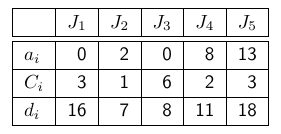
\includegraphics[height=0.2\paperheight]{./figures/3_tab.png}
\end{frame}

\begin{frame}{Task 3}{Earliest Deadline First}
  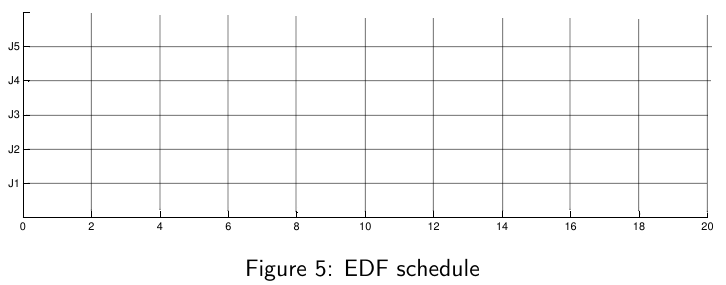
\includegraphics[width=\textwidth]{./figures/3_empty.png}
\end{frame}

\begin{frame}{Task 3}{Earliest Deadline First}
  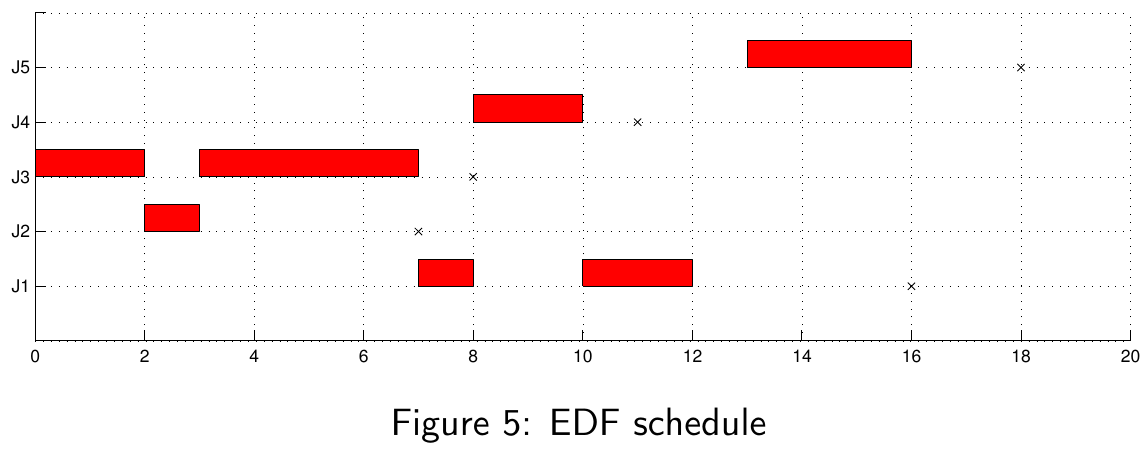
\includegraphics[width=\textwidth]{./figures/3_sol.png}
\end{frame}

\begin{frame}{Task 3}{Earliest Deadline First}
  \begin{task}
    \begin{itemize}
      \item at time $t = 3$, a new task $J_x$ arrives with execution time $C_x = 2$ and deadline $d_x = 10$.
      \item still \alert{guarantee the schedulability} of task set?
    \end{itemize}
  \end{task}
  \begin{requirements}
    \begin{itemize}
      \item $\forall i=1, \ldots, n \quad t+\sum_{k=1}^i c_k(t) \leq d_i$
    \end{itemize}
  \end{requirements}
\end{frame}

\if\preview0{
\begin{frame}{Task 3}{Earliest Deadline First}
  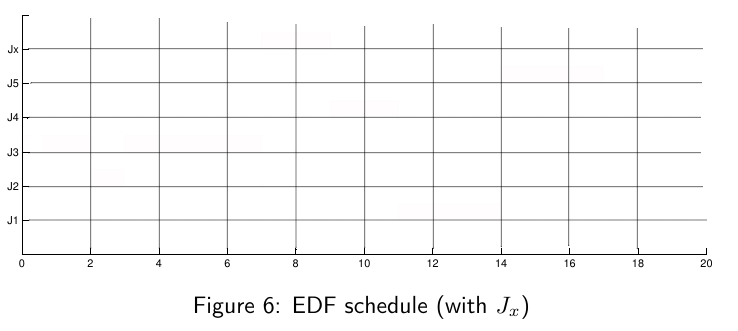
\includegraphics[width=\textwidth]{./figures/3_empty_2.png}
\end{frame}

\begin{frame}{Task 3}{Earliest Deadline First}
  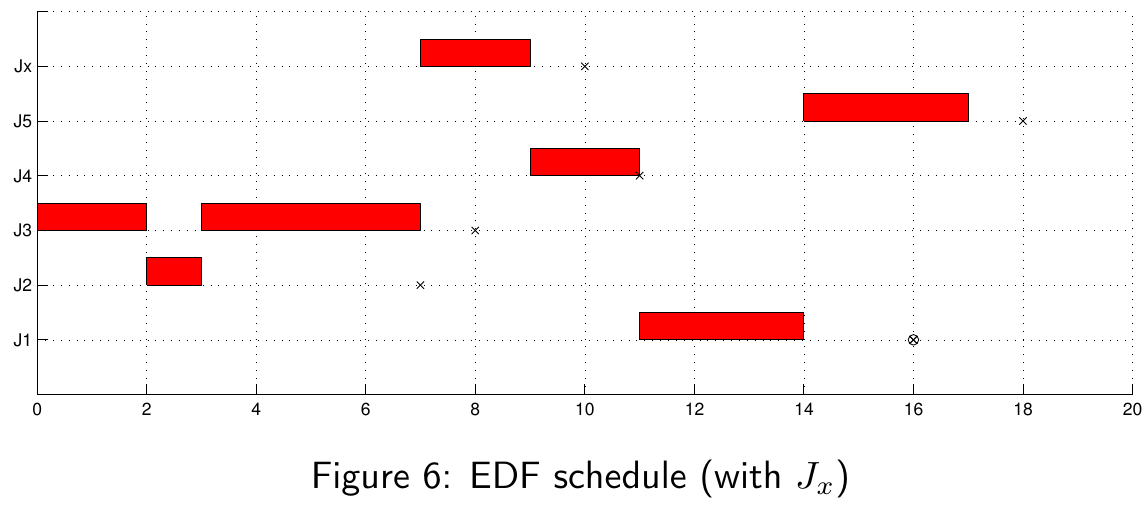
\includegraphics[width=\textwidth]{./figures/3_sol_2.png}
\end{frame}
}\fi
